\begin{frame}{Table of contents}
	\setbeamertemplate{section in toc}[sections numbered]
	\tableofcontents%[hideallsubsections]
\end{frame}

\section{Introduction}

\begin{frame}{Introduction}

	Curves have been interesting for a long time. Intuitively, a curve may be thought of as the trace left by a moving point. The first definition of a curve in the literature of mathematics appeared in Euclid's Elements.

	\begin{exampleblock}{}
	  	{\large ``The [curved] line is the first species of quantity, which has only one dimension, namely length, without any width nor depth, and is nothing else than the flow or run of the point which will leave from its imaginary moving some vestige in length, exempt of any width.''}
	  	\vskip5mm
	  	\hspace*\fill{\small--- Euclid's Elements}
	\end{exampleblock}

\end{frame}

\begin{frame}{Introduction}
	
	In modern mathematics, curves have various definitions depending on the settings they are in. In this setting, the main actor is the algebraic curves which are the zero set of polynomials defined over the field of complex numbers.

	An interesting question about curves is to find functions on them with prescribed zeroes and poles. The \textbf{Riemann-Roch theorem} finds the dimension of the space of such meromorphic functions. This theorem is a vital tool in the fields of complex analysis and algebraic geometry. It relates the complex analysis of a connected compact Riemann surface with the surface's purely topological property of genus, in a way that can be carried over into purely algebraic settings.

\end{frame}

\begin{frame}{Introduction - Riemann-Roch Theorem}

	\begin{theorem}[Riemann-Roch]
		Let $D$ be a divisor on a non-singular projective curve $\curveC$ in $\projective_2$ with genus $g$, $\kappa$ be a canonical divisor on $\curveC$.
		$$l(D)-l(\kappa-D)=\deg(D)-g+1$$
	\end{theorem}

\end{frame}

\begin{frame}{Introduction - Theorem Consequences and Other Proofs}

	The Riemann-Roch theorem has many very useful consequences including an easy proof of the law of associativity for the additive group structure on a non-singular cubic curve and a proof that every meromorphic function on a non-singular projective curve is rational.

	There are different ways to prove the Riemann–Roch Theorem. One way is to take an analytic approach and study holomorphic and meromorphic functions with Serre duality, which can be found in \cite{ref:miranda}. Another, more modern approach includes the concept of schemes and sheaf cohomology, and an example to this can be found in \cite{ref:hartshorne}. I have utilized resources \cite{ref:kirwan}, \cite{ref:fulton}, \cite{ref:keith}, \cite{ref:hampus}, \cite{ref:terrytao} to study the theorem. This paper uses a more elementary machinery to approach the Riemann-Roch theorem.

\end{frame}

\section{Preliminaries}

\begin{frame}{Preliminaries}

	In order to understand the statement and the proof of the Riemann–Roch theorem, one must first state several definitions and results.

\end{frame}

\subsection{Complex Curves}

\begin{frame}{Complex Algebraic Curves in $\CC^2$}

	A \vocab{complex algebraic curve} in $\CC^2$ is
	$$\curveC=\{(x,y)\in\CC^2:P(x,y)=0\}$$
	where $P(x,y)\in\CC[x,y]$ is a polynomial with no repeated factors.
	$$d=\max\{u+v:c_{u,v}\neq 0\}$$ where $\displaystyle P(x,y)=\sum_{u,v}c_{u,v}\,x^u\,y^v$ is called the \vocab{degree} of the curve.

\end{frame}

\begin{frame}{Hilbert's Nullstellensatz}
	
	The condition of no repeated factors is needed because of the following theorem.

	\begin{factx}[Hilbert's Nullstellensatz]
		For $P(x,y),Q(x,y)\in\CC[x,y]$, $\curveC_P=\curveC_Q$ if and only if $P$ and $Q$ have the same irreducible factors, possibly occuring with different multiplicities.
	\end{factx}

\end{frame}

\begin{frame}{Singularity, Multiplicity and Tangent Lines}
	
	$(a,b)\in\curveC$ is a \vocab{singularity} of $\curveC$ if $$\frac{\partial P}{\partial x}(a,b)=\frac{\partial P}{\partial y}(a,b)=0$$
	The \vocab{multiplicity} of $\curveC$ at $(a,b)\in\curveC$ is the smallest positive integer $m$ such that $$\frac{\partial^mP}{\partial x^i\partial y^j}(a,b)\neq 0$$ for some $i\geq 0$, $j\geq 0$ such that $i+j=m$. The Taylor polynomial $$\sum_{i+j=m}\frac{\partial^mP}{\partial x^i\partial y^j}(a,b)\frac{(x-a)^i(y-b)^j}{i!j!}$$ is then homogeneous of degree $m$ and its linear factors (homogeneous polynomials factor as a product of linear polynomials) are the tangent lines to $\curveC$ at $(a,b)$. If the factors of this polynomial are all different lines, than this singularity is \vocab{ordinary}.

\end{frame}

\begin{frame}{Example}
	
	The cubic curve (degree 3) defined by the polynomial $P(x,y)=x^3+x^2-y^2$ has a double point (a singularity of multiplicity 2) at the point $(0,0)$ which is ordinary.
	Although they are fundamentally different, the real algebraic curve counterpart has the following shape.
	\begin{center}
		\begin{tikzpicture}[scale=0.8]
			\draw[->] (-2.2, 0) -- (2.2, 0) node[right] {$x$};
			\draw[->] (0, -2.2) -- (0, 2.2) node[above] {$y$};
			\draw[scale=2.0, domain=-1:1, smooth, variable=\x, blue] plot (\x,{sqrt((\x*\x*(\x+1))});
			\draw[scale=2.0, domain=-1:1, smooth, variable=\x, blue] plot (\x,{-sqrt((\x*\x*(\x+1))});
		\end{tikzpicture}
	\end{center}

\end{frame}

\begin{frame}{Complex Projective Space}
	
	\vocab{Complex projective space} of dimension $n$, denoted $\projective_n$, is the set of complex one dimensional subspaces of the complex vector space $\CC^{n+1}$. $\projective_n$ can be identified with the set of equivalence classes for the equivalence relation $\sim$ on $\CNZ$ such that $a\sim b$ if there is some $\lambda\in\CC-\{0\}$ such that $a=\lambda b$. That is, every vector of $\CNZ$ represents an element $x$ of $\projective_n$
	$$\projective_n=\{[x_0,\cdots,x_n]:(x_0,\cdots,x_n)\in\CNZ\}$$
	such that
	$$[\lambda x_0,\lambda x_1,\cdots,\lambda x_n]\sim[x_0,x_1,\cdots,x_n]$$

\end{frame}

\begin{frame}{Complex Projective Space}
	
	\begin{remark}
		$\projective_n$ is $\CC^n$ with a copy of $\projective_{n-1}$ at infinity.
	\end{remark}

	\seprule

	\begin{itemize}
		\item Adding a point at infinity to the complex plane results in a space that is topologically a sphere. Hence the complex projective line, $\projective_1$, is also known as the Riemann sphere.
	\end{itemize}

\end{frame}

\begin{frame}{Complex Projective Curves in $\projective_2$}
	
	A \vocab{complex projective curve} in $\projective_2$ is
	$$\curveC=\{[x,y,z]\in \projective_2:P(x,y,z)=0\}$$
	where $P(x,y,z)\in\CC[x,y,z]$ is a non-constant homogeneous polynomial with no repeated factors. $d=\deg P$ is called the \vocab{degree} of the curve.

\end{frame}

\begin{frame}{Singularity, Multiplicity and Tangent Lines}
	
	$[a,b,c]\in\projective_2$ is a \vocab{singularity} of $\curveC$ if $$\frac{\partial P}{\partial x}(a,b,c)=\frac{\partial P}{\partial y}(a,b,c)=\frac{\partial P}{\partial z}(a,b,c)=0$$
	The \vocab{multiplicity} of $\curveC$ at $[a,b,c]\in\curveC$ is the smallest positive integer $m$ such that $$\frac{\partial^mP}{\partial x^i\partial y^j\partial z^k}(a,b,c)\neq 0$$ for some $i\geq 0$, $j\geq 0$, $k\geq 0$ such that $i+j+k=m$.
	Tangent line to $\curveC$ at a non-singular point $[a,b,c]$ is the line $$\frac{\partial P}{\partial x}(a,b,c)x+\frac{\partial P}{\partial y}(a,b,c)y+\frac{\partial P}{\partial z}(a,b,c)z=0$$

	\seprule

	\begin{itemize}
		\item The curve defined by $P(x,y,z)=y^2z-x^3$ has a singular point at $[0,0,1]$
	\end{itemize}

\end{frame}

\begin{frame}{Affine and Projective Curves}
	
	Complex affine curves and complex projective curves are different but closely related by the following lemma.

	\begin{lemma}\label<1>{lemma:affproj}
		Let $[a,b,c]$ be a point of the projective curve $$\tilde{\curveC}=\{[x,y,z]\in \projective_2:P(x,y,z)=0\}$$
		If $c\neq 0$, then $[a,b,c]$ is a non-singular point of $\tilde{\curveC}$ if and only if $\left(\frac{a}{c},\frac{b}{c}\right)$ is a non-singular point of the affine curve $$\curveC=\{(x,y)\in\CC^2:P(x,y,1)=0\}$$
	\end{lemma}

\end{frame}

\begin{frame}{Proof of Lemma \ref{lemma:affproj}}
	
	The point $\left(\frac{a}{c},\frac{b}{c}\right)$ is a singular point of $\curveC$ if and only if $$P\left(\frac{a}{c},\frac{b}{c},1\right)=0=\frac{\partial P}{\partial x}\left(\frac{a}{c},\frac{b}{c},1\right)=\frac{\partial P}{\partial y}\left(\frac{a}{c},\frac{b}{c},1\right)$$
	which by $P$ being homogeneous is equivalent to
	$$P(a,b,c)=0=\frac{\partial P}{\partial x}(a,b,c)=\frac{\partial P}{\partial y}(a,b,c)$$
	By the Euler relation given below
	$$x\frac{\partial P}{\partial x}(x,y,z)+y\frac{\partial P}{\partial y}(x,y,z)+z\frac{\partial P}{\partial z}(x,y,z)=dP(x,y,z)$$
	which can be obtained by differentiating
	$$P(\lambda x,\lambda y,\lambda z)=\lambda^dP(x,y,z)$$
	with respect to $\lambda$ and then setting $\lambda=1$, this happens when $\frac{\partial P}{\partial z}(a,b,c)=0$ also holds, i.e. $[a,b,c]$ is a singular point of $\tilde{\curveC}$.

\end{frame}

\subsection{Bezout Theorem}

\begin{frame}{Bezout Theorem}
	
	\begin{theorem}[Bezout]\label<1>{thm:bezout}
		$\curveC$ and $\curveD$ are complex projective curves of degrees $n$ and $m$ in $\projective_2$ which have no common component. $$\sum_{p\in \curveC\cap\curveD}I_p(\curveC,\curveD)=nm$$
	\end{theorem}

\end{frame}

\begin{frame}{Resultant}
	
	Let $$P(x)=\poly{a}{n},$$ $$Q(x)=\poly{b}{m},$$ be polynomials of degrees $n$ and $m$ in $\CC[x]$. The \vocab{resultant} $\resPQ$ is the determinant of the $n+m$ by $n+m$ matrix.

	For polynomials $$P(x,y,z)=\polyh{a}{n},$$ $$Q(x,y,z)=\polyh{b}{m},$$ the resultant $\resPQ(y,z)$ is defined similarly.

\end{frame}

\begin{frame}{Resultant Matrix}
	
	$$
	\begin{pmatrix}
		a_0 & a_1 & \cdots & a_n & 0 & 0 & & & \cdots & 0 \\
		0 & a_0 & a_1 & \cdots & a_n & 0 & & & \cdots & 0 \\
		\vdots & & & & & & & & & \vdots \\
		0 & 0 & \cdots & 0 & a_0 & a_1 & & & \cdots & a_n \\
		b_0 & b_1 & & \cdots & & b_m & 0 & & \cdots & 0 \\
		0 & b_0 & b_1 & & \cdots & & b_m & 0 & \cdots & 0 \\
		\vdots & & & & & & & & & \vdots \\
		0 & \cdots & 0 & b_0 & b_1 & & & & \cdots & b_m
	\end{pmatrix}
	$$

\end{frame}

\begin{frame}{Resultant Properties}
	
	\begin{itemize}
		\item If $P(x,y,z)$ and $Q(x,y,z)$ are homogeneous polynomials of degrees $n$ and $m$, then $\resPQ(y,z)$ is either identically 0 or a homogeneous polynomial of degree $nm$.
		
		\item Polynomials $P(x)$ and $Q(x)$ have a non-constant common factor if and only if $\resPQ=0$.
		
		\item Homogeneous polynomials $P(x,y,z)$ and $Q(x,y,z)$ have a non-constant common factor if and only if $\resPQ(y,z)\equiv 0$.
	
		\item If $P(x)=\prod_{i=0}^{n}x-\lambda_i$ and $Q(x)=\prod_{j=0}^{m}x-\mu_j$ then $$\resPQ=\prod_{0\leq i\leq n,0\leq j\leq m}\mu_j-\lambda_i$$
		In particular, $\mathcal{R}_{P,QR}=\mathcal{R}_{P,Q}\mathcal{R}_{P,R}$
	\end{itemize}

\end{frame}

\begin{frame}{Weak Form of Bezout Theorem}
	
	\begin{theorem}\label<1>{thm:weak_bezout}
		Any two projective curves $\curveC$ and $\curveD$ in $\projective_2$ of degrees $n$ and $m$ intersect in at least one point and at most $nm$ points if they have no common component.
	\end{theorem}

\end{frame}

\begin{frame}{Proof of Weak Form of Bezout Theorem}
	
	Let $\curveC$ and $\curveD$ are defined by homogeneous polynomials $P(x,y,z)$ and $Q(x,y,z)$ of degrees $n$ and $m$. The resultant $\resPQ(y,z)$ is a homogeneous polynomial of degree $nm$, so the product of $nm$ linear factors of the form $bz-cy$. For any factor of the form $bz-cy$, the resultant of polynomials $P(x,b,c)$ and $Q(x,b,c)$ in $x$ is identically 0. Therefore, there exists $a\in\CC$ such that $P(a,b,c)=Q(a,b,c)=0$. Since there is at least one such pair $(b,c)$, there is a point $[a,b,c]\in\curveC\cap\curveD$.

\end{frame}

\begin{frame}{Proof of Weak Form of Bezout Theorem (continued)}
	
	Now suppose that $\curveC$ and $\curveD$ have more than $nm$ intersections. Choose any finite set $S$ of distinct points in $\curveC\cap\curveD$ with more than $nm$ elements. By applying a suitable projective transformation, assume that $[1,0,0]$ is not on $\curveC$ or on $\curveD$ or on a line passing through two distinct points in $S$. For any intersection point, there must be a linear factor because $b$ and $c$ can not simultaneously be zero since $[1,0,0]$ is not an intersection point. Also, any two such linear factors are different because $[1,0,0]$ is not on a line passing through two intersection points. Hence, for any intersection point, $\resPQ(y,z)$ has a different linear factor but $\resPQ(y,z)$ with more than $nm$ linear factors must be identically zero.

\end{frame}

\begin{frame}{Intersection Multiplicity}

	There is a unique intersection multiplicity $I_P(\curveC,\curveD)$ defined for all projective curves $\curveC$, $\curveD$ in $\projective_2$ satisfying the following properties.
	\begin{itemize}
		\item $I_P(\curveC,\curveD)=I_P(\curveD,\curveC)$
		\item $I_P(\curveC,\curveD)=\infty$ if $P$ lies on a common component and otherwise $I_P(\curveC,\curveD)$ is a non-negative integer
		\item $I_P(\curveC,\curveD)=0$ if and only if $P\not\in\curveC\cap\curveD$
		\item Two distinct lines meet with intersection multiplicity of 1 at their unique point of intersection.
		\item If $\curveC:=P(x,y,z)$, $\curveC_1:=P_1(x,y,z)$, and $\curveC_2:=P_2(x,y,z)$ where $P(x,y,z)=P_1(x,y,z)P_2(x,y,z)$, then $I_P(\curveC,\curveD)=I_P(\curveC_1,\curveD)+I_P(\curveC_2,\curveD)$
		\item If $\curveC:=P(x,y,z)$, $\curveD:=Q(x,y,z)$ have degrees $n$ and $m$, and $\mathcal{E}:=PR+Q$ where $R(x,y,z)$ is of degree $m-n$, then $I_P(\curveC,\curveD)=I_P(\curveC,\mathcal{E})$
	\end{itemize}

\end{frame}

\begin{frame}{Intersection Multiplicity}

	Moreover, if $\curveC$ and $\curveD$ have no common component and by suitable selection $[1,0,0]$ does not belong to $\curveC\cap\curveD$, any line through two distinct points of $\curveC\cap\curveD$, or any tangent to $\curveC$ or $\curveD$ at a point of $\curveC\cap\curveD$, then $I_P(\curveC,\curveD)$ of any $P=[a,b,c]\in\curveC\cap\curveD$ is $\nu_{bz-cy}(\resPQ(y,z))$

\end{frame}

\begin{frame}{Proof of Bezout Theorem}
	
	The resultant can be express as
	$$\resPQ(y,z)=\prod_{i=0}^k(b_iz-c_iy)^{e_i}$$
	where $e_1+e_2+\cdots+e_k=nm$. By the arguments in the proof of the weak form of Bezout Theorem, $I_{P_i}(\curveC,\curveD)=e_i$.

\end{frame}

\subsection{Degree-Genus Formula for Non-singular Curves}

\begin{frame}{Degree-Genus Formula}
	
	A non-singular complex projective curve in $\projective_2$ is topologically a sphere with $g$ handles. This number $g$ is called the \vocab{genus} of the curve.
	
	\begin{theorem}[degree-genus formula]\label<1>{thm:degree_genus}
		For a non-singular complex projective curve of degree $d$ in $\projective_2$ with genus $g$, $$g=\frac{(d-1)(d-2)}{2}$$
	\end{theorem}

\end{frame}

\begin{frame}{Intuitive Proof of Degree-Genus Formula}

	Consider a singular complex projective curve $\curveC$ which is union of $d$ projective lines in general position i.e. no point lies on more than two lines. A complex projective line $L$ is homeomorphic to the two dimensional unit sphere $\mathbb{S}^2$ by the stereographic projection. So, $\curveC$ is homeomorphic to a union of $d$ spheres meeting in $\frac{d(d-1)}{2}$ points. It is possible to perturb the curve by a small amount to get a non-singular curve. This perturbation turns the $\frac{d(d-1)}{2}$ intersection points into handles expect for $d-1$ points which are used to join the $d$ spheres. Hence, the number of handles is $\frac{d(d-1)}{2}-(d-1)$.

\end{frame}

\subsection{Riemann Surfaces}

\begin{frame}{Riemann Surfaces}
	
	A \vocab{Riemann surface} is a connected complex one dimensional manifold which is locally homeomorphic to $\CC$ i.e any point has an open neighborhood homeomorphic to an open subset of $\CC$. The feature of Riemann surfaces that interests this paper the most is that it makes sense to do complex analysis and define holomorphic and meromorphic functions on them. A \vocab{holomorophic function} on a Riemann surface $S$ is a holomorphic map from $S$ to $\CC$ and a \vocab{meromorphic function} on $S$ is a holomorphic map from $S$ to $\overline{\CC}=\CC\cup\{\infty\}$. Sphere, torus, and the curves that this paper is dealing with are the most famous examples.

\end{frame}

\begin{frame}{Differentials}
	
	A \vocab{meromorphic differential} on $\curveC$ is a symbol $df$ which satisfies the following relations
	\begin{align*}
		d(f+g) &= df+dg\\
		d(fg) &= fdg+gdf\\
		da &= 0
	\end{align*}
	for any meromorphic functions $f$, $g$ on $\curveC$ and $a\in\CC$.

\end{frame}

\subsection{Divisors}

\begin{frame}{Divisors}
	
	A \vocab{divisor} $D$ on $\curveC$ is the formal sum $$D=\sum_{P\in\curveC}n_PP$$ such that $n_P\in\mathbb{Z}$ for every $P\in\curveC$ and $n_P=0$ for all but finitely many $p\in\curveC$.
	
	The \vocab{degree} of $D$ is then $$\deg(D)=\sum_{P\in\curveC}n_P$$ The set of all divisors on $\curveC$ is an Abelian group, denoted $\Div(\curveC)$, and the degree defines a homomorpism from $\Div(\curveC)$ to $\mathbb{Z}$.

\end{frame}

\begin{frame}{Effective Divisors}
	
	If $n_P\geq 0$ for all $P\in\curveC$, then $D$ is called \vocab{effective} and denoted $D\geq 0$. $D\geq D'$ if $D-D'\geq 0$. This also means $\deg(D)\geq\deg(D')$ 

\end{frame}

\begin{frame}{Principal Divisors}
	
	The divisor of a meromorphic function on $\curveC$
	$$(f)=\sum_{P\in\curveC}\ord_P(f)P$$
	is called a \vocab{principal divisor} where $\ord_P(f)$ is the order of zero (or the negative of the order of pole) at $P$. Two divisors $D$ and $D'$ are said to be \vocab{equivalent}, denoted $D\sim D'$, if $D-D'$ is a principal divisor.
	
	A principal divisor on $\curveC$ has degree zero. That is, any meromorphic function defined on $\curveC$ has the same number of zeros and poles, counted with multiplicities. Therefore, equivalent divisors have the same degree.

\end{frame}

\begin{frame}{Properties of Principal Divisors}
	
	\begin{minipage}{0.50\textwidth}
		\begin{align*}
			\ord_P(fg) &= \ord_P(f)+\ord_P(g) \\
			\ord_P\left(\frac{f}{g}\right) &= \ord_P(f)-\ord_P(g) \\
			\ord_P(f+g) &\geq \min(\ord_P(f),\ord_P(g))
		\end{align*}
	\end{minipage}
	\begin{minipage}{0.10\textwidth}
		$\implies$
	\end{minipage}
	\begin{minipage}{0.30\textwidth}
		\begin{align*}
			(fg) &= (f)+(g) \\
			\left(\frac{f}{g}\right) &= (f)-(g) \\
			(f+g) &\geq \min((f),(g))
		\end{align*}
	\end{minipage}

\end{frame}

\begin{frame}{Vector Space of Functions}
	
	Let $D=\sum_{P\in\curveC}n_PP$ be a divisor on $\curveC$, then $\mathcal{L}(D)$ is the set of meromorphic functions $f$ on $\curveC$ satisfying $(f)+D\geq 0$ together with the zero function. That is, a meromorphic function $f$ on $\curveC$ belongs to $\mathcal{L}(D)$ if $f$ is holomorphic except at those $P\in\curveC$ for which $n_P>0$ and there the order of the pole is at most $n_P$, and also $f$ has a zero of order at least $-n_P$ at every $P\in\curveC$ with $n_P<0$. By the properties of principal divisors, $\mathcal{L}(D)$ is a complex vector space. Denote $l(D)=\dim(\mathcal{L}(D))$.

	\seprule

	\begin{itemize}
		\item Let $D=2P_1-3P_2$. If $f\in\mathcal{L}(D)$, then it has a pole of order at most 2 at $P_1$ and a zero of order at least 3 at $P_2$.
	\end{itemize}

\end{frame}

\begin{frame}{Properties of $\mathcal{L}(D)$}
	
	\begin{factx}\label<1>{corollary:ldzero}
		If $\deg(D)<0$, then $l(D)=0$ because if $f$ is a meromorphic function on $\curveC$ such that $(f)+D\geq 0$, then $\deg(D)=\deg((f)+D)\geq 0$. Also, $\mathcal{L}(0)$ consists of only constant functions, so $l(0)=1$.
	\end{factx}

	\begin{factx}\label<1>{fact:ld12}
		If $D\sim D'$, then $l(D)=l(D')$ because if $D'=D+(g)$ where $g$ is a meromorphic function on $\curveC$, then $f\mapsto fg$ defines a isomorphism from $\mathcal{L}(D)$ to $\mathcal{L}(D')$. Also, if $D_1\leq D_2$, then $\mathcal{L}(D_1)\subset\mathcal{L}(D_2)$.
	\end{factx}

\end{frame}

\begin{frame}{Divisors}
	
	\begin{lemma}\label<1>{lemma:ldp}
		$0\leq l(D+P)-l(D)\leq 1$ for any divisor $D$ and point $P$ on $\curveC$.
	\end{lemma}
	
	By Fact \ref{fact:ld12}, $\mathcal{L}(D)\subset\mathcal{L}(D+P)$, so $0\leq l(D+P)-l(D)$. Take a function $t$ such that $\ord_P(t)=1$ (it is called uniformizer). Consider
	$$\phi:\mathcal{L}(D+P)\rightarrow \CC,\,f\mapsto (t^{n_P+1}f)(P)$$
	that maps $f$ to the evaluation of $t^{n_P+1}f$ at $P$. Since $\ord_P(t^{n_P+1}f)=n_P+1+\ord_P(f)\geq 0$ for a $f\in\mathcal{L}(D+P)$, $P$ is not a pole and $\phi$ is well-defined. $\ker(\phi)$ consists of functions that has a zero at $P$ i.e. $\ord_P(t^{n_P+1}f)=n_P+1+\ord_P(f)\geq 1$. This precisely describes the functions in $\mathcal{L}(D)$. Therefore,
	$$\mathcal{L}(D+P)/\mathcal{L}(D)\cong\CC$$
	and $\dim(\mathcal{L}(D+P)/\mathcal{L}(D))=l(D+P)-l(D)\leq 1$.

\end{frame}

\begin{frame}{Canonical Divisors}
	
	If $\omega$ is a meromorphic differential on $\curveC$ which is not identically zero, then we can define the divisor $(\omega)$ of $\omega$ similarly. The divisor of a meromorphic differential is called a \vocab{canonical divisor} and is denoted by $\kappa$. Any two canonical divisors are equivalent and have the same degree of $2g-2$ by Proposition 6.31 from \cite{ref:kirwan}.

\end{frame}

\section{Theorem Statement and Proof}

\begin{frame}{Theorem Statement}
	
	Let $D$ be a divisor on a non-singular projective curve $\curveC$ in $\projective_2$ with genus $g$, $\kappa$ be a canonical divisor on $\curveC$, and $P$ be a point on $\curveC$.

\end{frame}

\begin{frame}{Lemmas for the Riemann-Roch Theorem}
	
	\begin{lemma}\label<1>{lemma:ld_ldp}
		$$0\leq l(D)-l(D-P)+l(\kappa-D+P)-l(\kappa-D)\leq 1$$
	\end{lemma}
	
	By Lemma \ref{lemma:ldp}, assume simultaneously $l(D)-l(D-P)=1$ and $l(\kappa-D+P)-l(\kappa-D)=1$. Then there exists $f\in\mathcal{L}(D)-\mathcal{L}(D-P)$ and $g\in\mathcal{L}(\kappa-D+P)-\mathcal{L}(\kappa-D)$. So, $(f)+D\geq 0$ and $(g)+\kappa-D+P\geq 0$. These inequalities are actually equalities at point $P$. Adding the inequalities having this in mind, one gets $(fg)+\kappa+P\geq 0$ with an equality at $P$. So, $fg\in\mathcal{L}(\kappa+P)-\mathcal{L}(\kappa)$. This is a contradiction since $\mathcal{L}(\kappa+P)-\mathcal{L}(\kappa)=\varnothing$ by Proposition 5.15 from \cite{ref:hampus}.

\end{frame}

\begin{frame}{Lemmas for the Riemann-Roch Theorem}
	
	\begin{lemma}[Riemann's Inequality]\label<1>{lemma:halfrr}
		$$l(D)-l(\kappa-D)\geq\deg(D)+1-g$$
	\end{lemma}
	
	Let $L(x,y,z)$ define a line in $\projective_2$ and let
	$$H=\sum_{P\in\curveC}I_P(\curveC,L)P$$
	be a divisor of degree $d$ by Bezout theorem (Theorem \ref{thm:bezout}). $\deg(\kappa-mH)=\deg(\kappa)-md$ and this is negative for large enough $m$. By Corollary \ref{corollary:ldzero}, $l(\kappa-mH)=0$. For a homogeneous polynomial $Q(x,y,z)$ of degree $m$,
	$$\frac{Q(x,y,z)}{L(x,y,z)^m}$$
	defines a meromorphic function $f$ that satisfies $(f)+mH\geq 0$ i.e. an element of $\mathcal{L}(mH)$.

\end{frame}

\begin{frame}{Lemmas for the Riemann-Roch Theorem}
	
	For any such $Q(x,y,z)$, a function $f$ can be obtained but $Q'(x,y,z)=Q(x,y,z)+P(x,y,z)R(x,y,z)$ gives the same function $f$ for any homogeneous polynomial $R(x,y,z)$ of degree $m-d$. Hence, if $\CC_t[x,y,z]$ defines the space of homogeneous polynomials of degree $t$ whose dimension is easily found to be $|\{x^iy^jz^k:i+j+k=t\}|={t+2 \choose 2}=\frac{(t+1)(t+2)}{2}$, then
	\begin{align*}
		l(mH) &\geq \dim(\CC_m[x,y,z]/P(x,y,z)\CC_{m-d}[x,y,z])\\
		&= \dim(\CC_m[x,y,z])-\dim(\CC_{m-d}[x,y,z])\\
		&= \frac{(m+1)(m+2)}{2}-\frac{(m-d+1)(m-d+2)}{2}\\
		&= md-g+1\\
		&= \deg(mH)-g+1
	\end{align*}
	by the degree-genus formula (Theorem \ref{thm:degree_genus}). Thus, the lemma holds for $D=mH$ when $m$ is large enough.

\end{frame}

\begin{frame}{Lemmas for the Riemann-Roch Theorem}
	
	Now, the aim is, for any divisor $D=\sum_{P\in\curveC}n_PP$, and $m_0$, to find a $m\geq m_0$ and not necessarily distinct points $P_1,P_2,\cdots,P_k\in\curveC$ such that 
	$$D+P_1+P_2+\cdots+P_k\sim mH$$
	By adding points, $n_P\geq 0$ can be assumed. For each of the finitely many $P$ such that $n_P>0$, take a line through $P$ that intersects $\curveC$ at points (possibly with multiplicities) $Q_{1,P},Q_{2,P},\cdots,Q_{d,P}$. Since the ratio of any two linear homogeneous polynomials defines a meromorphic function, for any $P$, $$Q_{1,P}+Q_{2,P}+\cdots+Q_{d,P}\sim H$$
	Taking $m=\deg(D)$,
	$$mH\sim \sum_{n_P>0}n_P\sum_{i=1}^dQ_{i,P}= D+P_1+P_2+\cdots+P_k$$
	for $k=md-m$.

\end{frame}

\begin{frame}{Lemmas for the Riemann-Roch Theorem}
	
	So, by a simple induction on Lemma \ref{lemma:ld_ldp} and the results proven so far
	\begin{align*}
		l(D)-l(\kappa-D) &\geq l(D+P_1+P_2+\cdots+P_k)-l(\kappa-D-P_1-P_2-\cdots-P_k)-k\\
		&= l(mH)-l(\kappa-mH)-k\\
		&\geq \deg(mH)-g+1-k\\
		&= \deg(D+P_1+P_2+\cdots+P_k)-g+1-k\\
		&= \deg(D)-g+1
	\end{align*}
	as $l(mH)\geq\deg(mH)-g+1$ and $l(\kappa-mH)=0$.

\end{frame}

\begin{frame}[standout,plain]

	Now comes the main theorem that turns this inequality into an equality.
	
\end{frame}

\begin{frame}{Riemann-Roch Theorem}
	
	\begin{theorem}[Riemann-Roch]\label<1>{thm:rr}
		$$l(D)-l(\kappa-D)=\deg(D)-g+1$$
	\end{theorem}

\end{frame}

\begin{frame}{Proof of Riemann-Roch Theorem}
	
	Apply Lemma \ref{lemma:halfrr} for $D$ and $\kappa-D$ respectively to obtain
	$$l(D)-l(\kappa-D)\geq\deg(D)-g+1$$
	and
	\begin{align*}
		l(\kappa-D)-l(D) &\geq\deg(\kappa-D)-g+1\\
		&= \deg(\kappa)-\deg(D)-g+1\\
		&= 2g-2-\deg(D)-g+1\\
		&= -\deg(D)+g-1
	\end{align*}
	since $\deg(\kappa)=2g-2$.

\end{frame}

\section{Applications}

\begin{frame}{Applications - Degree versus Dimension of Vector Space}
	
	The relation between $\deg(D)$ and $l(D)$ for a curve of genus $g$ can be partially determined by the Riemann-Roch theorem (Theorem \ref{thm:rr}). $l(D)$ of a divisor of negative degree is 0 by Corollary \ref{corollary:ldzero}. For divisors $D$ with $\deg(D)>2g-2$, one gets $l(D)=\deg(D)-g+1$ since $l(\kappa-D)=0$ again by Corollary \ref{corollary:ldzero}. For each additional point added to $D$, $l(D)$ either stays the same or increases by 1 by Lemma \ref{lemma:ldp}. So, the graph of $\deg(D)$ versus $l(D)$ in $\mathbb{Z}\times\mathbb{Z}$ would look like Figure \ref{fig:degdld}, where the gray region represents the possibilities.

\end{frame}

\begin{frame}{Applications - Degree versus Dimension of Vector Space}
	
	\begin{figure}
		\centering
		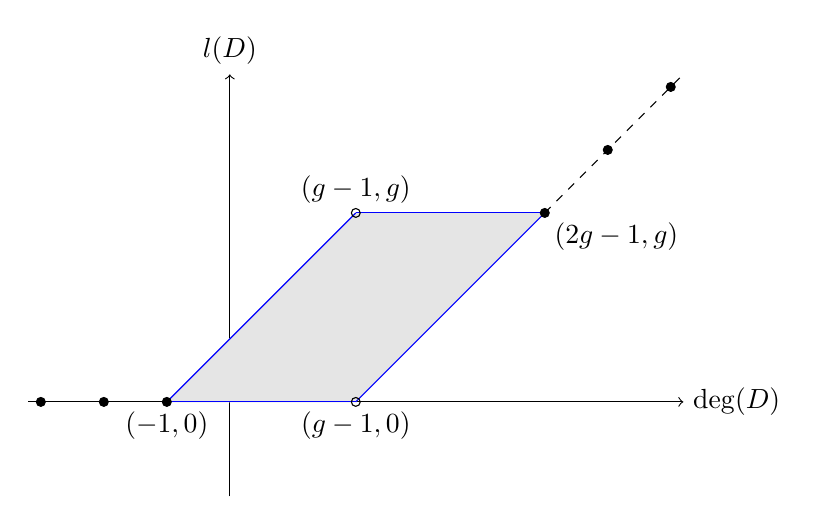
\begin{tikzpicture}[scale=0.8]
			\draw[->] (-3.2, 0) -- (7.2, 0) node[right] {$\deg(D)$};
			\draw[->] (0, -1.5) -- (0, 5.2) node[above] {$l(D)$};
			\filldraw[gray!20] (-1,0) -- (2,0) -- (5,3) -- (2,3) -- (-1,0);
			\draw[scale=1.0, domain=2:5, smooth, variable=\x, blue] plot ({\x}, {\x-2});
			\draw[scale=1.0, domain=-1:2, smooth, variable=\x, blue] plot ({\x}, {\x+1});
			\draw[scale=1.0, domain=2:5, smooth, variable=\x, blue] plot ({\x}, {3});
			\draw[scale=1.0, domain=-1:2, smooth, variable=\x, blue] plot ({\x}, {0});
			\filldraw[black] (-1,0) circle (2pt) node[anchor=north]{$(-1,0)$};
			\filldraw[black] (-2,0) circle (2pt) node[anchor=west]{};
			\filldraw[black] (-3,0) circle (2pt) node[anchor=west]{};
			\filldraw[black] (5,3) circle (2pt) node[anchor=north west]{$(2g-1,g)$};
			\filldraw[black] (6,4) circle (2pt) node[anchor=west]{};
			\filldraw[black] (7,5) circle (2pt) node[anchor=west]{};
			\draw[] (2,0) circle (2pt) node[anchor=north]{$(g-1,0)$};
			\draw[] (2,3) circle (2pt) node[anchor=south]{$(g-1,g)$};
			\draw[dashed] (5,3) -- (7.2,5.2);
		\end{tikzpicture}
		\caption{Graph of $\deg(D)$ versus $l(D)$ for a curve with genus $g$}
		\label<1>{fig:degdld}
	\end{figure}

\end{frame}

\begin{frame}{Applications - Group Structure of Curves}
	
	\begin{theorem}[Group Structure of Curves]\label<1>{thm:group}
		Let $\curveC$ be a non-singular projective curve of degree $3$ in $\projective_2$. Let $O$ be an inflection point of $\curveC$. There is a unique additive group structure on $\curveC$ such that $O$ is the zero element and for any $P,Q,R\in\curveC$,
		$$P+Q+R=0$$
		if and only if $P$, $Q$, $R$ are the three points of intersection of a line with $\curveC$.
	\end{theorem}

\end{frame}

\begin{frame}{Applications - Proof of the Existence of a Group Structure of Curves}
	
	$-O=O$ and for $P\neq O$, $-P$ is the other intersection of the line through $P$ and $O$. And $P+Q=-R$ where $R$ is the other intersection of the line through $P$ and $Q$. Therefore, if there is a structure, it is unique. Commutativity is inherent from the definition of the operation.
	
	For the associativity, let
	\begin{align*}
		A &= P+Q\\
		B &= A+R\\
		C &= Q+R\\
		D &= P+C
	\end{align*}
	and show that $B=D$.

\end{frame}

\begin{frame}{Applications - Proof of the Existence of a Group Structure of Curves}
	
	There is a linear polynomial that vanishes at $P$, $Q$, $-A$. The ratio of this polynomial to the polynomial that vanishes at $A$, $-A$, $O$ defines a meromorphic function $\phi_A$ with zeroes at $P$, $Q$ and poles at $A$, $O$. Similarly, $\phi_B$ can be obtained with zeroes at $A$, $R$ and poles at $B$, $O$. Then, $\phi_A\phi_B$ is a meromorphic function with zeroes at $P$, $Q$, $R$ and poles at $B$, $O$, $O$. Doing this for $C$ and $D$, one obtains a meromorphic function $\phi_C\phi_D$ with zeroes at $P$, $Q$, $R$ and poles at $D$, $O$, $O$. The ratio of $\phi_C\phi_D$ and $\phi_A\phi_B$ has a simple zero at $D$ and a simple pole at $B$. By the Riemann-Roch theorem  (\ref{thm:rr}),
	$$l(B)-l(\kappa-B)=\deg(B)-g+1$$
	$l(\kappa-B)=0$ since $\deg(\kappa-B)=\deg(\kappa)-\deg(B)=-1<0$. So, $l(B)=1$. That is, the only meromorphic functions on $\curveC$ with at most a simple pole at $B$ are the constant functions. Therefore, $B=D$.

\end{frame}

\begin{frame}{Applications - Group Structure of Curves}
	
	\begin{figure}
		\centering
		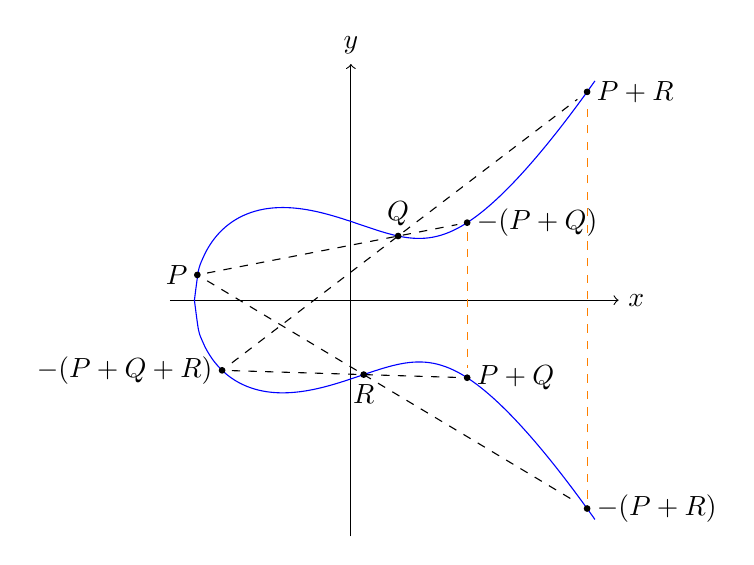
\begin{tikzpicture}[scale=1.0]
			\draw[->] (-2.3, 0) -- (3.4, 0) node[right] {$x$};
			\draw[->] (0, -3.0) -- (0, 3.0) node[above] {$y$};
			\draw[domain=-1.987076:3.1,samples=100,smooth,variable=\x,blue] plot ({\x},{sqrt((\x^3)/3.375 - (\x)/1.5 + 1)});
			\draw[domain=-1.987076:3.1,samples=100,smooth,variable=\x,blue] plot ({\x},{-sqrt((\x^3)/3.375 - (\x)/1.5 + 1)});
			\node (P) at (-1.95, 0.321) {};
			\node (Q) at (0.6, 0.81486) {};
			\node (R) at (0.16233, -0.945) {};
			\node (NPR) at (3.0, -2.64575) {};
			\node (PR) at (3.0, 2.64575) {};
			\node (NPQ) at (1.47657, 0.98463) {};
			\node (PQ) at (1.47657, -0.98463) {};
			\node (NPQR) at (-1.63584, -0.8908) {};
			\filldraw[black] (P) circle (1pt) node[anchor=east]{$P$};
			\filldraw[black] (Q) circle (1pt) node[anchor=south]{$Q$};
			\filldraw[black] (R) circle (1pt) node[anchor=north]{$R$};
			\filldraw[black] (NPR) circle (1pt) node[anchor=west]{$-(P+R)$};
			\filldraw[black] (PR) circle (1pt) node[anchor=west]{$P+R$};
			\filldraw[black] (NPQ) circle (1pt) node[anchor=west]{$-(P+Q)$};
			\filldraw[black] (PQ) circle (1pt) node[anchor=west]{$P+Q$};
			\filldraw[black] (NPQR) circle (1pt) node[anchor=east]{$-(P+Q+R)$};
			\draw[dashed] (P) -- (NPQ);
			\draw[dashed] (P) -- (NPR);
			\draw[dashed, color=orange] (NPQ) -- (PQ);
			\draw[dashed, color=orange] (NPR) -- (PR);
			\draw[dashed] (NPQR) -- (PQ);
			\draw[dashed] (NPQR) -- (PR);
		\end{tikzpicture}
		\caption{Associativity of the elliptic curve group operation}
		\label<1>{fig:ec}
	\end{figure}

\end{frame}

\begin{frame}{Applications}

	\begin{remark}
		Theorem \ref{thm:group}, for a finite field instead of $\CC$, is what makes elliptic curve cryptography possible, which is an integral part of the modern cryptology.
	\end{remark}

\end{frame}

% \begin{frame}
% 	Frame without a title
% 	\begin{alertblock}{Important theorem}
% 		Sample text in red box
% 	\end{alertblock}
% \end{frame}

% \begin{frame}{Blocks}
% 	Three different block environments are pre-defined and may be styled with an
% 	optional background color. % \cite{Knuth92}
	
% 	\begin{columns}[T,onlytextwidth]
% 		\column{0.45\textwidth}
% 		\begin{block}{Default}
% 			Block content.
% 		\end{block}
		
% 		\begin{alertblock}{Alert}
% 			Block content.
% 		\end{alertblock}
		
% 		\begin{exampleblock}{Example}
% 			Block content.
% 		\end{exampleblock}
		
% 		\column{0.45\textwidth}
		
% 		\metroset{block=fill}
		
% 		\begin{block}{Default}
% 			Block content.
% 		\end{block}
		
% 		\begin{alertblock}{Alert}
% 			Block content.
% 		\end{alertblock}
		
% 		\begin{exampleblock}{Example}
% 			Block content.
% 		\end{exampleblock}
		
% 	\end{columns}
% \end{frame}

\appendix

\begin{frame}[allowframebreaks]{References}
	\begin{thebibliography}{9}
    \bibitem{ref:miranda} \textbf{Algebraic Curves and Riemann Surfaces}, by Rick Miranda.
    \bibitem{ref:hartshorne} \textbf{Algebraic Geometry}, by Robert Hartshorne.
    \bibitem{ref:kirwan} \textbf{Complex Algebraic Curves}, by Frances Kirwan.
    \bibitem{ref:fulton} \textbf{Algebraic Curves}, by William Fulton.
    \bibitem{ref:keith} \textbf{Elementary Algebraic Geometry}, by Keith Kendig.
    \bibitem{ref:hampus} \textbf{Elementary Proof of Riemann-Roch Theorem}, by Hampus Sundgren.
    \bibitem{ref:terrytao} \textbf{\href{https://terrytao.wordpress.com/2018/03/28/246c-notes-1-meromorphic-functions-on-riemann-surfaces-and-the-riemann-roch-theorem/}{Blog of Terence Tao}}
\end{thebibliography}

\end{frame}
